\chapter{Scalar Equations} \label{ch:2ScalarEqns}
In this chapter we look at scalar wave equations in our waveguide-like geometry, treating the cross-sectional structure as singular.
We base our approach largely off the work of Zhikov \cite{zhikov2000extension}, in that we consider what can be colloquially described as ``differential equations with respect to a measure $\dddmes$".
We will give a rigorous definition of the kinds of problems and spaces that this colloquialism covers in the following sections.
The purpose of this chapter is to highlight the techniques that are available to us, and how we shall adapt them for the more descriptive (or physical) vector systems we consider in chapter \ref{ch:3VectorEqns}.
We will also highlight some of the details that must be considered when taking this approach; however do not extensively work to fill in these details here - this will again be done when we consider vector systems.

\section{The Scalar Sobolev Spaces} \label{sec:ScalarSobSpaces}
In this section we look to construct the function spaces that we shall be working with throughout the chapter.
What we present is a synopsis of the work of Zhikov presented in \tstk{cite his (2?) papers?}, although with an adapted notation to suit our needs and with an omission of some details - the interested reader is directed to the references provided. 
Let $n\in\naturals$, $D\subset\reals^n$ and $\nu$ be a (Borel) measure on $D$.
Denote the set of smooth functions on $D$ by $\smooth{D}$, and then let $W=W\bracs{D,\mathrm{d}\nu}$ be the closure of the set of pairs $\bracs{\phi,\grad\phi}$ in $\ltwo{D}{\nu}\times\ltwo{D}{\nu}^n$ where $\phi\in\smooth{D}$.
That is
\begin{align*}
	W = W\bracs{D,\nu} &= \overline{\clbracs{\bracs{\phi,\grad\phi} \ \vert \ \phi\in\smooth{D}}} \quad \text{in} \ \ltwo{D}{\nu}\times\ltwo{D}{\nu}^n.
\end{align*}
An element of $W$ is a pair $\bracs{u,z}$; we denote the component $z$ by $z=\grad_\nu u$ and refer to it as a ``gradient of $u$ with respect to $\nu$", although as we shall shortly discuss this terminology requires some qualification.
The Sobolev space $\gradSob{D}{\nu}$ is then the collection of first components $u$,
\begin{align*}
	\gradSob{D}{\nu} &= \clbracs{u \ \vert \ \bracs{u,z}\in W}.
\end{align*}

An important feature to note about $\gradSob{D}{\nu}$ is that any of its elements $u$ can (and indeed will) have multiple gradients with respect to $\nu$.
That is to say that there will be multiple (distinct) functions $z\in\ltwo{D}{\nu}^n$ such that $\bracs{u,z}\in W$.
Indeed if we have that $\bracs{u,z}\in W$ and $\bracs{0,y}\in W$, then we clearly have that $\bracs{u,z+y}\in W$ as well.
This hints at the possibility that any $\grad_\nu u$ can be written as the sum of a gradient (with respect to $\nu$) of the zero function and a function that is orthogonal (in the $L^2$-norm) to the set of gradients (with respect to $\nu$) of zero.
Denoting by $\gradZero{D}{\nu}$ the set of gradients (with respect to $\nu$) of the zero function,
\begin{align*}
	\gradZero{D}{\nu} = \clbracs{z \ \vert \ \bracs{0,z}\in W},
\end{align*}
this is to claim that for any $u\in\gradSob{D}{\nu}$,
\begin{align*} \labelthis\label{eq:OrthogonalGradExpression}
	\grad_\nu u &= g_\perp + g,
\end{align*}
where $g\in\gradZero{D}{\nu}$ and $g_\perp \perp \gradZero{D}{\nu}$.
Indeed Zhikov \cite{zhikov2000extension} provides a stronger assertion that this; for each $u\in\gradSob{D}{\nu}$ there exists a unique $g_\perp \perp \gradZero{D}{\nu}$ such that for any $\grad_\nu u$ there exists some $g\in\gradZero{D}{\nu}$ such that \eqref{eq:OrthogonalGradExpression} holds.
Namely there is precisely one function $g_\perp$ that results in \eqref{eq:OrthogonalGradExpression} holding, regardless of which gradient (with respect to $\nu$) of $u$ we consider (the element $g\in\gradZero{D}{\nu}$ is of course what changes depending on the considered gradient). \tstk{it would be good to provide an overview of the argument Zhikov employs to prove this.}
This argument can be taken further to show that for any elliptic $n\times n$ matrix $A$, there is a unique $g_\perp$ such that $Ag_\perp \perp \gradZero{D}{\nu}$ - this extension is useful for discussing the so-called ``differential equations with respect to $\nu$", which we now turn our attention to. \newline

Now that we have a concept of gradient with respect to $\nu$, it makes sense to discuss equations involving this object.
For a function $f\in\ltwo{D}{\nu}$ and elliptic matrix $A$, we say that the pair $\bracs{u,\grad_\nu u}$ with $u\in\gradSob{D}{\nu}$ is a solution to the (elliptic) equation
\begin{align} \label{eq:GeneralScalarStrongForm}
	-\grad_\nu \cdot \bracs{A(x)\grad_\nu u(x)} &= f(x) \quad x\in D
\end{align}
if (and only if)
\begin{align} \label{eq:GeneralScalarWeakForm}
	\integral{D}{A\grad_\nu u \cdot \phi}{\nu} &= \integral{D}{f\phi}{\nu} \quad \forall \phi\in\smooth{D}.
\end{align}
One can draw analogues between the pair of equations \eqref{eq:GeneralScalarWeakForm},\eqref{eq:GeneralScalarStrongForm} and the strong and weak form of an ODE - indeed when $\nu$ is Lebesgue measure this is precisely what is happening.
For general $\nu$ we do not necessarily have integration by parts, and so we can only refer to \eqref{eq:GeneralScalarWeakForm} as the ```weak form" of \eqref{eq:GeneralScalarStrongForm} formally.
Moreover, \eqref{eq:GeneralScalarWeakForm} is the only way for us to assign a meaning to ```solutions to \eqref{eq:GeneralScalarStrongForm}"; the solution as a pair is also required due to the earlier discussion of gradients of $u\in\gradSob{D}{\nu}$.
That being said, existence and uniqueness of the solution pair $\bracs{u,\grad_\nu u}$ is guaranteed by appealing to the Riesz representation theorem and the bilinear form defined by \eqref{eq:GeneralScalarWeakForm}.
One can \tstk{again, give synopsis of Zhikov} importantly establish that the $\grad_\nu u$ in the solution pair coincides with the unique gradient of $u$ such that $A\grad_\nu u \perp \gradZero{D}{\nu}$; which means that understanding $\gradZero{D}{\nu}$ is crucial to determining solutions to \eqref{eq:GeneralScalarStrongForm}.
One other property of $\gradZero{D}{\nu}$ that is worth noting is that it is a closed linear subspace of $\ltwo{D}{\nu}^n$; which is something we will exploit when looking into the structure of these spaces in the example that follows.

\section{An Example System} \label{sec:ScalarExample}
To compliment the theory outlined in section \ref{sec:ScalarSobSpaces}, and to highlight some of the considerations we shall be taking forward, we now provide some analysis of an example system.
Let $\ddom\subset\reals^2$ be a bounded domain and $\graph = \bracs{V,E}$ be a finite graph embedded in $\ddom$.
By this we associate each vertex $v_i\in V$ with a point $\vec{v}_i\in\reals^2$, and each edge $\bracs{v_i,v_j}\in E$ to the segment $I_{ij}=\sqbracs{\vec{v}_i,\vec{v}_j}$.
In a slight abuse of notation we drop the distinction between the vertices $v_i$ of $\graph$ and their associated points $\vec{v}_i\in\ddom$, and simply use the notation $v_i$ for both objects.
Similarly we adopt the notation $I_{ij}$ for both the edges of $\graph$ and their associated segments in $\ddom$.
Because of the embedding we can also consider $\graph$ as a subset of $\ddom$ itself, and so can make sense of expressions like $\graph\cap[0,1]^2$ by interpreting $\graph$ as the intersection of its segments $I_{ij}$. 
On $\ddom$ we define the measure $\ddmes$ as the measure which supports 1D Lebesgue measure on the edges of $\graph$, so for some $B\subset\ddom$ we have that 
\begin{align*}
	\ddmes\bracs{B} = \sum_{I_{ij}\in E}\lambda_{ij}\bracs{B \cap I_{ij}}
\end{align*}
where $\lambda_{ij}$ is the measure on $\reals^2$ that supports 1D Lebesgue measure down the edge $I_{ij}$. 
We are interested in the (spectral) problem
\begin{align} \label{eq:ScalarExampleStrongForm}
	-\grad_\ddmes \cdot \grad_\ddmes u &= \omega^2 u
\end{align}
for $u\in\gradSob{\ddom}{\ddmes}$, and recovering the spectrum ($\omega^2$) values of the operator that gives rise to this problem.
\tstk{the provisos about considering the spectral problem, and the things we will have to consider in the vector case. This should include how we have already taken the Fourier transform of the 3D problem, and the Gelfand transform, and how this is the $k=0,\theta=0$ case - $\theta$ the quasi-momentum.}

To see how the setup just detailed relates to the wave propagation problems that we wish to consider in future, see figure \ref{fig:ScalarStrucDiagram}.
We interpret $\ddom$ as being the period cell of the cross-section of some waveguide that extends into 3D, whose waveguide axis is parallel to the $x_3$-axis.
The graph $\graph$ represents the (singular) structure within the period cell that is invariant down the waveguide, and the measure $\ddmes$ indicates that we are interested wave propagation on (the planes included by) $\graph$ only\footnote{Later we will look to relate singular structure problems such as this to thin-structure problems, where the cross section has a graph-like structure but with edges of non-zero ``thickness".}.
\begin{figure}[h!]
	\centering
	\begin{tikzpicture}
		%actual waveguide
		\begin{scope}[shift={(5,-2)}]
			\draw (0,0) rectangle (2,2);
			\node[anchor=south] at (1,1) {$\ddom\subset\reals^2$};
			%waveguide axis
			\draw[red] (2,0) -- (2+3.5/2,1);
			\draw[dashed, red] (0,0) -- (3.5/2,1);
			\draw[red] (0,2) -- (3.5/2,3);
			\draw[red] (2,2) -- (2+3.5/2,3);
		\end{scope}		
		
		%axes labels
		\begin{scope}[shift={(5,2)}, scale=0.75]
			\draw[->] (0,1) -- (2,1) node[anchor=west] {$x_1$};
			\draw[->] (0,1) -- (0,3) node[anchor=south] {$x_2$};
			\draw[->] (0,1) -- (2,1+8/7) node[anchor=south west] {$x_3$};
		\end{scope}
		
		%graph stucture
		\begin{scope}[shift={(-3,-1.25)}]
			\draw (0,0) rectangle (5,5);
			%graph edges
			\draw (2.5,2.5) -- (4,3) -- (4.5,4);
			\draw (2.5,2.5) -- (0.5,4.5);
			\draw (2.5,2.5) -- (1,1) -- (3.5,1) -- (4,2) -- cycle;
			%nodes
			\filldraw (2.5,2.5) circle (1pt) node[anchor=south] {$v_i$};	
			\filldraw (4,3) circle (1pt);	\filldraw (4.5,4) circle (1pt);
			\filldraw (0.5,4.5) circle (1pt) node[anchor=north east] {$v_j$};
			\filldraw (1,1) circle (1pt);	\filldraw (3.5,1) circle (1pt);	\filldraw (4,2) circle (1pt);
			\node[anchor=south] at (2.5,5) {$\graph\subset\ddom$};
			%labelling for I_ij
			\node[anchor=north east] at (1.5,3.5) {$I_{ij}$};
			\draw[->] (2,3.2) -- (1.5,3.7) node[anchor=west] {$e_{ij}$};
		\end{scope}
		
		%lines between waveguide pic and graph illustration
		\draw[dashed, blue] (5,-2) -- (-3,-1.25);
		\draw[dashed, blue] (7,-2) -- (2,-1.25);
		\draw[dashed, blue] (7,0) -- (2,3.75);
		\draw[dashed, blue] (5,0) -- (-3,3.75);
	\end{tikzpicture}
	\caption{\label{fig:ScalarStrucDiagram} An illustration of the wider setting for $\ddom$ with singular structure. The 2D problem will arise from considering a structure that is periodic in the $\bracs{x_1,x_2}$-plane and translation invariant in the $x_3$ direction; and taking the (Fourier and) Gelfand transforms to arrive at a family of problems posed on the 2D-period (cross-section) period cell.}
\end{figure}

\subsection{Analysis of $\gradZero{\ddom}{\ddmes}$}
We first pursue an understanding of $\gradZero{\ddom}{\ddmes}$, as this will be crucial for helping us reduce the problem \eqref{eq:ScalarExampleStrongForm} to something more manageable.
We begin by first considering what $\gradZero{\ddom}{\ddmes}$ looks like when the $\graph$ consists of only a single edge $I$ parallel to the $x_1$-axis.
In this case $\ddmes = \lambda_I$ (Lebesgue measure down $I$) and it can be deduced that 
\begin{align*}
	\gradZero{\ddom}{\lambda_I} &= 
	\clbracs{
		\begin{pmatrix} 0 \\ f	\end{pmatrix}
		\ \vert \ f\in\ltwo{\ddom}{\ddmes}
	},
\end{align*}
see for example \cite{zhikov2000extension}.
Intuitively we can think of this result as follows: the smooth gradient $\grad$ (from which $\grad_\ddmes$ is constructed) details the rate of change of the function it is applied to.
The measure $\ddmes$ however can only ``see" along (or alternatively ``only cares about") what's going on along the segment $I$, as this is it's entire support.
As such $\ddmes$ can only see the change along the segment $I$, and hence we find that $\gradZero{\ddom}{\ddmes}$ consists of all the gradients that are directed perpendicular to $I$.
Furthermore any gradient orthogonal to $\gradZero{\ddom}{\ddmes}$ is directed parallel to $I$, so $\grad_\ddmes$ can only ``see" rates of change parallel to the segment $I$.
This interpretation is further reinforced by the following analysis, which characterises $\gradZero{\ddom}{\ddmes}$ when the segment $I$ is not (necessarily) parallel to the $x_1$-axis. \newline

Consider the case when $\graph$ consists of a single segment $I\subset\ddom$ with orthogonal co-ordinate system $y=\bracs{y_1,y_2}$, with $y_1$ parallel to $I$.
Let $R$ be the orthogonal change of co-ordinates $x=Ry$ with $x=\bracs{x_1,x_2}$ the orthogonal co-ordinate system along the axes.
Then if $v\in\gradZero{\ddom}{\lambda_I}$ then there exists a sequence of functions $\phi_k\in\smooth{\ddom}$ such that $\phi_k\lconv{\ltwo{\ddom}{\lambda_I}}0$ and $\grad_y\phi_k\lconv{\ltwo{\ddom}{\lambda_I}^2} v \toInfty{k}$.
Define $\psi_k = \phi_k\bracs{R^{\top}x}$, and let $\lambda_{R^{\top}I}$ denote the measure obtained from the composition $\lambda_I\circ R^{\top}$ (note that this is just the measure that supports 1D Lebesgue measure down the rotated segment).
Then using the change of variables $x=Ry$, $\psi_k\lconv{\ltwo{\ddom}{\lambda_{R^{\top}I}}}0$, and
\begin{align*}
	\grad_x\psi_k &= \grad_x\phi_k\bracs{R^{\top}x} = R^{\top}\grad_y\phi_k\bracs{y}\big\vert_{y=R^{\top}x} \\
	&\lconv{\ltwo{\ddom}{\lambda_{R^{\top}I}}} R^{\top}v\bracs{R^{\top}x} =: w\bracs{x}.
\end{align*}
Now $w$ is a gradient of zero for a segment parallel to the $x_1$ axis, and hence has the form
\begin{align*}
	w &= \begin{pmatrix} 0 \\ f \end{pmatrix}, &\quad f\in\ltwo{\ddom}{\lambda_{R^{\top}I}} \\
	\Leftrightarrow v\bracs{R^{\top}x} &= R\begin{pmatrix} 0 \\ f \end{pmatrix} &\\
	\Leftrightarrow v\bracs{y} &= R\begin{pmatrix} 0 \\ \widetilde{f} \end{pmatrix}, &\quad \widetilde{f}\in\ltwo{\ddom}{\lambda_I}.
\end{align*}
This confirms that 
\begin{align*}
	\gradZero{\ddom}{\lambda_I} &= \clbracs{R\begin{pmatrix} 0 \\ \widetilde{f} \end{pmatrix} \ \vert \ \widetilde{f}\in\ltwo{\ddom}{\lambda_I}} \\
	&= \clbracs{g\in\ltwo{\ddom}{\lambda_I}^2 \ \vert \ g\cdot e_{I} = 0}
\end{align*}
where $e_I$ is the unit vector directed along the segment $I$.

\subsubsection{Graphs with Multiple Edges}
Of course the results so far only describe the set of gradients of zero for graphs with single edges, however we can use this understanding of single edges to build up an understanding of what happens to gradients of zero when we have a more interesting graph.
In particular, we want to show that for a (multiple-edge) graph $\graph$ and $\ddmes$ supporting it's edges, we have that
\begin{align*}
	\gradZero{\ddom}{\ddmes} &= \clbracs{g\in\ltwo{\ddom}{\ddmes} \ \vert \ g\vert_{I_{ij}}\cdot e_{ij}=0 \ \forall I_{ij}\in E}.
\end{align*}
This provides an edge-wise characterisation of the set of gradients of zero; any gradient of zero for the whole graph has (upon restriction) the same form as a gradient of zero along each edge of the graph.
Here $g\vert_{I_{ij}}$ denotes the restriction of the function $g$ to the edge $I_{ij}$, and $e_{ij}$ denotes the unit vector (directed $v_i$ to $v_j$) along $I_{ij}$.
For convenience, we denote the set on the right hand side of the equality by $B$.
The inclusion $\gradZero{\ddom}{\ddmes} \subset B$ follows quickly:
\begin{prop} \label{prop:Grad0IncB}
	For $B=\clbracs{g\in\ltwo{\ddom}{\ddmes} \ \vert \ g\vert_{I_{ij}}\cdot e_{ij}=0 \ \forall I_{ij}\in E}$, we have
	\begin{align*}
		\gradZero{\ddom}{\ddmes}\subset B
	\end{align*}
\end{prop}
\begin{proof}
	If $g\in\gradZero{\ddom}{\ddmes}$ then there exists a sequence of smooth functions $\phi_k$ such that $\phi_k\lconv{\ltwo{\ddom}{\ddmes}}0, \grad\phi_k\lconv{\ltwo{\ddom}{\ddmes}^2}g$.
	Thus, due to the structure of $\ddmes$
	\begin{align*}
		\sum_{I_{ij}}\integral{I_{ij}}{\abs{\phi_k}^2}{\lambda_{I_{ij}}} &= \integral{\ddom}{\abs{\phi_k}^2}{\ddmes} \\
		&\rightarrow 0 \toInfty{k}
	\end{align*}
	and as every term in the sum is non-negative, each term must also be tending to 0.
	Thus 
	\begin{align*}
		\phi_k\lconv{\ltwo{\ddom}{\lambda_{I_{ij}}}}0 \ \forall I_{ij}\in E.
	\end{align*}
	Similarly
	\begin{align*}
		\sum_{I_{ij}}\integral{I_{ij}}{\abs{\grad\phi_k - g\vert_{I_{ij}}}^2}{\lambda_{I_{ij}}} &= \integral{\ddom}{\abs{\grad\phi_k - g}^2}{\ddmes} \\
		&\rightarrow 0 \toInfty{k}
	\end{align*}	
	and hence 
	\begin{align*}
		\grad\phi_k\lconv{\ltwo{\ddom}{\lambda_{I_{ij}}}^2} g\vert_{I_{ij}} \ \forall I_{ij}\in E.
	\end{align*}
	Hence $g\in B$.
\end{proof}

The reverse inclusion requires some further preliminary results before it can be proven.
\begin{lemma}[Extension of Gradients on Segments to Whole Graph] \label{lem:SegGradExtend}
	Let $I_{ij}^{n} = \clbracs{x\in I_{ij} \ \vert \ \mathrm{dist}\bracs{x, \partial I_{ij}}\geq\recip{n}}$.
	Suppose further that we have a function $g\in\ltwo{\ddom}{\ddmes}$ with $g=0$ on $\graph\setminus I_{ij}^{n}$ and $g\cdot e_{ij}=0$ on $I_{ij}^{n}$.
	Then $g\in\gradZero{\ddom}{\ddmes}$.
\end{lemma}
\begin{proof}
	As $g\cdot e_{ij}=0$ on $I_{ij}^{n}$ and $g=0$ on $I_{ij}\setminus I_{ij}^{n}$, we have that $g\cdot e_{ij}=0$ on $I_{ij}$ and hence $g\in\gradZero{\ddom}{\lambda_{I_{ij}}}$.
	So we can find a sequence of smooth functions $\phi_k$ with the properties $\phi_k\lconv{\ltwo{\ddom}{\lambda_{I_{ij}}}}0$, $\grad\phi_k\lconv{\ltwo{\ddom}{\lambda_{I_{ij}}}^2}g\vert_{I_{ij}}$.
	Now let $\chi_{ij}^{n}\in\smooth{\ddom}$ be the function such that
	\begin{align*}
		\chi_{ij}^{n}\bracs{x} &\in [0,1], \\
		\chi_{ij}^{n} = 1 &\text{ whenever } \mathrm{dist}\bracs{x, I_{ij}^n}\leq \recip{3n} \\
		\chi_{ij}^{n} = 0 &\text{ whenever } \mathrm{dist}\bracs{x, I_{ij}^n}\geq \frac{2}{3n}
	\end{align*}
	\begin{figure}
		\centering
		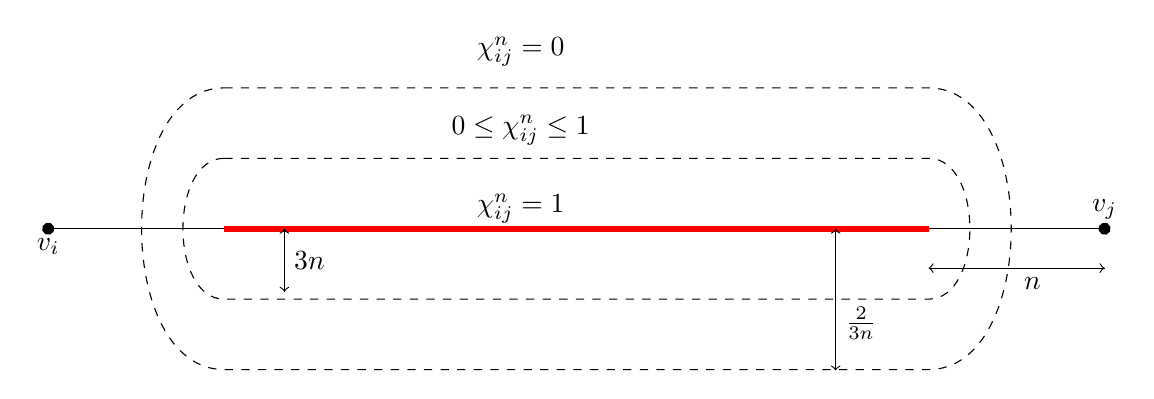
\begin{tikzpicture}
			\begin{scope}[scale=2, rotate=-26.565]
				\draw (0,0) -- (6,3);
				\filldraw (0,0) circle (1pt) node[anchor=north] {$v_i$};
				\filldraw (6,3) circle (1pt) node[anchor=south] {$v_j$};
				\draw[red, line width=2pt] (1,0.5) -- (5,2.5);
				\draw[dashed] (1-1/5,0.5+2/5) -- (5-1/5,2.5+2/5) to[out=26.565, in=26.565] (5+1/5,2.5-2/5) -- (1+1/5,0.5-2/5) to[out=180+26.565, in=180+26.565] cycle;
				\draw[dashed] (1-2/5,0.5+4/5) -- (5-2/5,2.5+4/5) to[out=26.565, in=26.565] (5+2/5,2.5-4/5) -- (1+2/5,0.5-4/5) to[out=180+26.565, in=180+26.565] cycle;
			\end{scope}
			\node at (6,0.25) {$\chi_{ij}^{n}=1$};
			\node at (6,1.25) {$0\leq\chi_{ij}^{n}\leq1$};
			\node at (6,2.25) {$\chi_{ij}^{n}=0$};
			\draw[->] (3,0) -- (3,-4/5);
			\draw[->] (3,-4/5) -- (3,0);
			\node[anchor=west] at (3,-2/5) {$\recip{3n}$};
			\node[anchor=west] at (10,-6/5) {$\frac{2}{3n}$};
			\draw[->] (10,0) -- (10,-9/5);
			\draw[->] (10,-9/5) -- (10,0);
			\draw[->] (13.416,-0.5) -- (11.18,-0.5);
			\draw[->] (11.18,-0.5) -- (13.416,-0.5);
			\node[anchor=north] at (12.5,-0.5) {$\recip{n}$};
		\end{tikzpicture}
		\caption{\label{fig:chiDiagram} The function $\chi_{ij}^n$ on the region surrounding the segment $I_{ij}^n$. Should another edge of $\graph$ lie in the region $\clbracs{x \ \vert \ \mathrm{dist}\bracs{x,I_{ij}^{n}}\leq\frac{2}{3n}}$, we can simply apply a rescaling to the argument of $\chi_{ij}^n$ to avoid this issue.}
	\end{figure}
	Note that since $\graph$ is finite, we can assume without loss of generality that the only edge of $\graph$ that lies in the support of $\chi_{ij}^n$ is $I_{ij}$, otherwise we apply a scaling to the argument of $\chi_{ij}^n$ to avoid this issue.
	Furthermore, $\abs{\grad\chi_{ij}^{n}}$ is bounded by a constant that depends on $n$ only.
	Now consider the sequence $\psi_k = \chi_{ij}^{n}\phi_k$.
	We have that
	\begin{align*}
		\integral{\ddom}{\abs{\psi_k}^2}{\ddmes} = \integral{I_{ij}}{\abs{\chi_{ij}^{n}\phi_k}^2}{\lambda_{I_{ij}}}
		\leq \integral{I_{ij}}{\abs{\phi_k}^2}{\lambda_{I_{ij}}} \rightarrow0 \toInfty{k},
	\end{align*}
	which is one of the desired convergence results for $\psi_k$.
	For the other convergence result we need, observe that
	\begin{align*}
		\integral{\ddom}{\abs{\phi_k\grad\chi_{ij}^{n}}^2}{\ddmes} &= \integral{I_{ij}}{\abs{\phi_k\grad\chi_{ij}^{n}}^2}{\lambda_{I_{ij}}} \\
		&\leq \sup_{I_{ij}}\bracs{\abs{\grad\chi_{ij}^{n}}^{2}}\integral{I_{ij}}{\abs{\phi_{k}}^{2}}{\ddmes} \\
		&\rightarrow 0 \toInfty{k}
	\end{align*}
	because $\abs{\grad\chi_{ij}^{n}}$ depends on $n$ only.
	Additionally
	\begin{align*}
		\integral{\ddom}{\abs{\chi_{ij}^n\grad\phi_k - g\vert_{I_{ij}}}^2}{\ddmes} &= \integral{I_{ij}}{\abs{\chi_{ij}^n\grad\phi_k - g\vert_{I_{ij}}}^2}{\lambda_{I_{ij}}} \\
		&= \integral{I_{ij}\setminus I_{ij}^n}{\abs{\chi_{ij}^n\grad\phi_k - g\vert_{I_{ij}}}^2}{\lambda_{I_{ij}}} + \integral{I_{ij}^n}{\abs{\chi_{ij}^n\grad\phi_k - g\vert_{I_{ij}}}^2}{\lambda_{I_{ij}}} \\
		&= \integral{I_{ij}\setminus I_{ij}^n}{\abs{\chi_{ij}^n\grad\phi_k}^2}{\lambda_{I_{ij}}} +  \integral{I_{ij}^n}{\abs{\grad\phi_k - g\vert_{I_{ij}}}^2}{\lambda_{I_{ij}}} \\
		&\leq \integral{I_{ij}\setminus I_{ij}^n}{\abs{\grad\phi_k}^2}{\lambda_{I_{ij}}} +  \integral{I_{ij}^n}{\abs{\grad\phi_k - g\vert_{I_{ij}}}^2}{\lambda_{I_{ij}}} \\
		&= \integral{I_{ij}\setminus I_{ij}^n}{\abs{\grad\phi_k - g\vert_{I_{ij}}}^2}{\lambda_{I_{ij}}} +  \integral{I_{ij}^n}{\abs{\grad\phi_k - g\vert_{I_{ij}}}^2}{\lambda_{I_{ij}}} \\
		&= \integral{I_{ij}}{\abs{\grad\phi_k - g\vert_{I_{ij}}}^2}{\lambda_{I_{ij}}} \rightarrow0 \toInfty{k},
	\end{align*}
	where we have made use of the fact that $g\vert_{I_{ij}}=0$ on $I_{ij}\setminus I_{ij}^n$ and the various properties of $\chi_{ij}^n$.
	Armed with these inequalities, we have that
	\begin{align*}
		\integral{\ddom}{\abs{\grad\psi_k - g\vert_{I_{ij}}}^2}{\ddmes} &= \integral{\ddom}{\abs{\chi_{ij}^n\grad\phi_k + \phi_k\grad\chi_{ij}^n - g\vert_{I_{ij}}}^2}{\ddmes} \\
		&\leq 2\integral{\ddom}{\abs{\phi_k\grad\chi_{ij}^n}^2}{\ddmes} + 2\integral{\ddom}{\abs{\chi_{ij}^n\grad\phi_k - g\vert_{I_{ij}}}^2}{\ddmes} \\
		&\rightarrow0 \toInfty{k}.
	\end{align*}
	Thus, $\psi_k$ is a sequence of smooth functions such that
	\begin{align*}
		\psi_k \lconv{\ltwo{\ddom}{\ddmes}} 0, &\quad
		\grad\psi_k \lconv{\ltwo{\ddom}{\ddmes}^2} g
	\end{align*}
	and hence, $g\in\gradZero{\ddom}{\ddmes}$.
\end{proof}

The other result we need is a convergence result for a particular form of function we will utilise in the proof.
Let the function $\eta\in\smooth{\ddom}$ with the properties
\begin{align*}
	\eta\bracs{x} &\in [0,1], \\
	\eta = 0 &\text{ whenever } \abs{x}\leq 1, \\
	\eta = 1 &\text{ whenever } \abs{x}\geq 2.
\end{align*}
Then for each $v_i\in V$ and $n\in\naturals$, we define
\begin{align*}
	\eta_i\bracs{x} = \eta\bracs{x-v_i}, &\quad \eta_i^n\bracs{x} = \eta_i\bracs{nx}
\end{align*}
which are clearly both smooth functions by composition.
\begin{lemma}[Convergence of $\eta_i^n$ in $\ltwo{\ddom}{\ddmes}$] \label{lem:etaConv}
	For any $v_i\in V$, $\eta_i^n \rightarrow 1$ in $\ltwo{\ddom}{\ddmes} \toInfty{n}$.
\end{lemma}
\begin{proof}
	We can directly prove this convergence by estimating the integral from above:
	\begin{align*}
		\begin{split}
			\integral{\ddom}{\abs{\eta_i^n-1}^2}{\ddmes} &= \integral{\graph\setminus B_{2/n}\bracs{v_{i}}}{\abs{\eta_{i}^{n}-1}^{2}}{\ddmes} + \integral{\graph \cap \bracs{B_{2/n}\bracs{v_{i}} \setminus B_{1/n}\bracs{v_{i}}}}{\abs{\eta_{i}^{n}-1}^{2}}{\ddmes} \\ + &\integral{\graph\cap B_{1/n}\bracs{v_{i}}}{\abs{\eta_{i}^{n}-1}^{2}}{\ddmes} \\
			&= \integral{\graph\setminus B_{2/n}\bracs{v_{i}}}{0}{\ddmes} + \integral{\graph \cap \bracs{B_{2/n}\bracs{v_{i}} \setminus B_{1/n}\bracs{v_{i}}}}{\abs{\eta_{i}^{n}-1}^{2}}{\ddmes} \\ + &\integral{\graph\cap B_{1/n}\bracs{v_{i}}}{}{\ddmes} \\
			&\leq \integral{\graph \cap \bracs{B_{2/n}\bracs{v_{i}} \setminus B_{1/n}\bracs{v_{i}}}}{}{\ddmes} + \integral{\graph\cap B_{1/n}\bracs{v_{i}}}{}{\ddmes} \\
			&=\integral{\graph\cap B_{2/n}\bracs{v_{i}}}{}{\ddmes} = \ddmes\bracs{\graph\cap B_{2/n}\bracs{v_{i}}} \\
			&\leq \frac{4 \abs{E}}{n} \rightarrow0 \toInfty{n}.
		\end{split}
	\end{align*}
	The last line following because each edge of $\graph$ can intersect $B_{2/n}\bracs{v_i}$ on a segment of length $\leq\frac{4}{n}$.
\end{proof}

We are now ready to prove that $B\subset\gradZero{\ddom}{\ddmes}$.
\begin{prop} \label{prop:BIncGrad0}
	For $B=\clbracs{g\in\ltwo{\ddom}{\ddmes} \ \vert \ g\vert_{I_{ij}}\cdot e_{ij}=0 \ \forall I_{ij}\in E}$, we have
	\begin{align*}
		B \subset \gradZero{\ddom}{\ddmes}
	\end{align*}
\end{prop}
\begin{proof}
	Take $g\in B$, and define a family of functions $g_{n}$ by
	\begin{align*}
		g_{n}\bracs{x} &= \recip{2}\sum_{i\in V}\sum_{i\sim j}\eta_{i}^{n}\bracs{x}\eta_{j}^{n}\bracs{x}g\vert_{I_{ij}}\bracs{x}
	\end{align*}
	where the notation $i\sim j$ means that there is an edge $(i,j)\in E$, and the sum is taken over such edges.
	Recall that $\graph$ was assumed finite, so there are no convergence issues with the double sum.
	Then for each $i,j$ with $i\sim j$, the function $\eta_{i}^{n}\eta_{j}^{n}g\vert_{I_{ij}}$ satisfies the hypothesis of \ref{lem:SegGradExtend}, so $\eta_{i}^{n}\eta_{j}^{n}g\vert_{I_{ij}}\in\gradZero{\ddom}{\ddmes}$.
	Furthermore, as $\gradZero{\ddom}{\ddmes}$ is a linear subspace of $\ltwo{\ddom}{\ddmes}^{2}$, $g_{n}\in\gradZero{\ddom}{\ddmes}$ too, for all $n$.
	By closure of $\gradZero{\ddom}{\ddmes}$; $g_{n}$ converges in $\gradZero{\ddom}{\ddmes}$ provided it converges at all, so it remains to show that $g_{n}\lconv{\ltwo{\ddom}{\ddmes}^2} g \toInfty{n}$.
	However with the result of \ref{lem:etaConv}, we have that $\eta_{i}^{n}\eta_{j}^{n}g\vert_{I_{ij}}\lconv{\ltwo{\ddom}{\ddmes}^2} g\vert_{I_{ij}}$ and hence
	\begin{align*}
		g_{n} \lconv{\ltwo{\ddom}{\ddmes}^2} &\recip{2}\sum_{i\in V}\sum_{j\sim i}g\vert_{I_{ij}} = g \toInfty{n},
	\end{align*}
	so $g\in\gradZero{\ddom}{\ddmes}$.
\end{proof}

\subsection{Reduction to a system of scalar equations} \label{sec:ScalarReduceEdgeEqns}
We now turn our attention back to \eqref{eq:ScalarExampleStrongForm}.
Recall that we interpret this in the weak sense, namely a pair $\bracs{u,\grad_\ddmes u}$ solves \eqref{eq:ScalarExampleStrongForm} if and only if
\begin{align} \label{eq:ScalarExampleWeakForm}
	\integral{\ddom}{\grad_\ddmes u \cdot \grad\phi}{\ddmes} &= \omega^2\integral{\ddom}{u\phi}{\ddmes} \quad \forall\phi\in\smooth{\ddom}.
\end{align}
\tstk{again reiterate Gelfand/Fourier and the case we are considering. Also how can we guarantee solutions to this system?}
We want to find an alternative but equivalent system to \eqref{eq:ScalarExampleWeakForm} that we can use in numerical schemes (as the measure $\ddmes$ prevents implementations via finite elements, for example) or is more tractable to an analytic approach.
To this end we look to work from \eqref{eq:ScalarExampleWeakForm} and employ our previous analysis to find an alternative problem. \newline

We begin by re-writing \eqref{eq:ScalarExampleWeakForm} by appealing to the nature of $\ddmes$;
\begin{align} \label{eq:ScalarExampleSumOfInts}
	0 &= \recip{2}\sum_{I_{ij}\in E}\integral{\ddom}{\grad_\ddmes u \cdot \grad\phi - \omega^2 u\phi}{\lambda_{ij}}.
\end{align}
Note that $I_{ij},I_{ji}\in E$ are the same edge of the graph $\graph$, which is what gives us the factor of a half.
Of course we may simply drop this factor of a half, and understand the sum as being over unique edges, which we henceforth do.
Next recall the notation introduced for the edge $I_{ij}$; we denote by $e_{ij}$ the unit vector along $I_{ij}$ pointing from $v_i$ to $v_j$,
\begin{align*}
	e_{ij} = \frac{v_j-v_i}{\norm{v_j-v_i}_2}.
\end{align*}
We define the map 
\begin{align*}
	r_{ij}:\sqbracs{0,\abs{I_{ij}}} &\rightarrow I_{ij}, \\
	r_{ij}\bracs{t} &= v_i + te_{ij}
\end{align*}
so $r'\bracs{t}=e_{ij}$.
Note that $r$ is therefore an admissible change of variables from $\sqbracs{0,\abs{I_{ij}}}$ to $I_{ij}$.
To prevent cluttered notation, we use an overhead tilde to denote composition with $r_{ij}$, so for example $\tilde{\phi}=\phi\circ r_{ij}$.
We next look at how to deal with each integral term.
Without loss of generality we can assume that each $I_{ij}$ is parallel to the $x_1$-axis by performing a rotation, and we denote by $u_{ij}\in\ltwo{\ddom}{\lambda_{ij}}$ the function such that $u_{ij}=u$ on the (potentially rotated) edge $I_{ij}$.
$u_{ij}$ can be thought of as the $ij$\textsuperscript{th}-part of $u$, or the part of $u$ down the edge $I_{ij}$ - this separation of $u$ onto separate functions on the edges of $\graph$ will prove useful in what follows.
Although we do not need to make this simplification since we have information about $\gradZero{\ddom}{\lambda_{ij}}$, it is helpful to do so in the following analysis.
In fact the information about $\gradZero{\ddom}{\lambda_{ij}}$ is necessary to perform the rotation we would use, and retain equivalence of the resulting problem to the original. \newline

With this simplification, we examine the term
\begin{align*}
	\integral{\ddom}{\grad_\ddmes u_{ij}\cdot\grad\phi}{\lambda_{ij}}.
\end{align*}
We know that the solution to \eqref{eq:ScalarExampleWeakForm} satisfies $\grad_\ddmes u \perp \gradZero{\ddom}{\ddmes}$ and so $\grad_\ddmes u_{ij} \perp \gradZero{\ddom}{\lambda_{ij}}$ by our analysis of gradients of zero.
Thus let us suppose that $\grad_\ddmes u_{ij} = \bracs{\alpha, \beta}^{\top}$.
Recalling the characterisation of $\gradZero{\ddom}{\lambda_{ij}}$ when $I_{ij}$ is parallel to the $x_1$-axis, we require that
\begin{align*}
	0 &= \integral{\ddom}{\grad_\ddmes u_{ij} \cdot \begin{pmatrix} 0 \\ f \end{pmatrix}}{\lambda_{ij}} \quad \forall f\in\ltwo{\ddom}{\lambda_{ij}}, \\
	\Rightarrow 0 &= \integral{I_{ij}}{\beta f}{\lambda_{ij}}
	= \int_{0}^{\abs{I_{ij}}}\widetilde{\beta}\widetilde{f}\md t.
\end{align*}
As $\widetilde{f}$ is arbitrary, we conclude that $\widetilde{\beta}=0$ and hence $\beta=0$.
Thus $\grad_\ddmes u_{ij} = \bracs{\alpha, 0}^{\top}$; we now show that $\alpha$ is related to the distributional derivative of the function $\widetilde{u}_{ij}$.
Notice that for any smooth function $\phi$ we have that
\begin{align*} \labelthis\label{eq:PartialToTDiff}
	\partial_t\widetilde{\phi}(t) &= \grad\phi\bracs{r_{ij}(t)}\cdot r'_{ij}(t) = \partial_1\phi\bracs{r_{ij}(t)} \\
	&= \widetilde{\partial_1\phi}(t),
\end{align*}
as $r'_{ij}=e_{ij}=\bracs{1,0}^{\top}$.
Now as $u_{ij}\in\ltwo{\ddom}{\lambda_{ij}}$ we can find smooth functions $\alpha_n$ such that
\begin{align*}
	\alpha_n\lconv{\ltwo{\ddom}{\lambda_{ij}}}u_{ij}, \quad \grad\alpha_n\lconv{\ltwo{\ddom}{\lambda_{ij}}^2}\begin{pmatrix} \alpha \\ 0	\end{pmatrix}.
\end{align*}
Exploiting the change of variables $r_{ij}$ and writing these statements using integrals converging in $\reals$ implies
\begin{align*}
	\int_0^{\abs{I_{ij}}}\abs{\widetilde{\alpha}-\widetilde{u}_{ij}}^2 \md t &\rightarrow 0, \\
	\int_0^{\abs{I_{ij}}}\abs{\partial_t\widetilde{\alpha}_n - \widetilde{\alpha}}^2 \md t = \int_0^{\abs{I_{ij}}}\abs{\partial_1\widetilde{\alpha}_n - \widetilde{\alpha}}^2 \md t &\rightarrow 0, \\
	\int_0^{\abs{I_{ij}}}\abs{\partial_2\widetilde{\alpha}_n}^2 \md t &\rightarrow 0, \toInfty{n}.
\end{align*}
In particular the first two convergences imply that $\widetilde{\alpha}=\widetilde{u}'_{ij}$; that is that $\widetilde{\alpha}$ is the distributional derivative of $\widetilde{u}_{ij}\in\gradSob{\sqbracs{0,\abs{I_{ij}}}}{t}$.
Using the notation $u'_{ij}$ for the $\ltwo{\ddom}{\lambda_{ij}}$ function such that $u'_{ij} = \widetilde{u}'_{ij}\circ r_{ij}^{-1}$, we can write $\grad_\ddmes u_{ij} = \bracs{u'_{ij}, 0}^{\top}$.
In light of this we see that
\begin{align*}
	\integral{\ddom}{\grad_\ddmes u_{ij} \cdot \grad\phi - \omega^2 u_{ij}\phi}{\lambda_{ij}}
	&= \int_0^{\abs{I_{ij}}}\widetilde{u}'_{ij}\widetilde{\phi}' - \omega^2\widetilde{u}_{ij}\widetilde{\phi} \md t.
\end{align*}

Equipped with this knowledge, we are able to transform \eqref{eq:ScalarExampleSumOfInts} into
\begin{align} \label{eq:ScalarExampleLebesgueIntegrals}
	0 &= \sum_{I_{ij}\in E}\int_0^{\abs{I_{ij}}}\widetilde{u}'_{ij}\widetilde{\phi}' - \omega^2\widetilde{u}_{ij}\widetilde{\phi} \md t.
\end{align}
The choice of $\phi$ was arbitrary so in particular \eqref{eq:ScalarExampleLebesgueIntegrals} must hold when $\mathrm{supp}\bracs{\phi}$ contains precisely one edge $I_{ij}$, meaning that we have
\begin{align*}
	0 &= \int_0^{\abs{I_{ij}}}\widetilde{u}'_{ij}\widetilde{\phi}' - \omega^2\widetilde{u}_{ij}\widetilde{\phi} \md t, \quad \forall I_{ij}\in E, \ \forall \phi\in\smooth{\ddom}.
\end{align*}
That is to say, we have arrived at a system of differential equations (``edge equations") for $\widetilde{u}_{ij}$ (the ``edge solutions").
This weak formulation admits numerical solution by (for example) finite elements, providing us with a method to recover the original function $u$.
If we assume more regularly of $u$, for example assume that $u\in C^2\bracs{\ddom}$ so the second derivative of $u$ exists in the strong sense we can obtain a system of ODEs in the edge solutions $\widetilde{u}_{ij}$, complete with boundary conditions.
We obtain one (second-order) differential equation for each edge $I_{ij}$ by integrating each edge equation by parts;
\begin{align*}
	0 &= \int_0^{\abs{I_{ij}}}\widetilde{u}'_{ij}\widetilde{\phi}' - \omega^2\widetilde{u}_{ij}\widetilde{\phi} \md t, \quad \forall\phi\in\smooth{\ddom} \\
	&= \int_0^{\abs{I_{ij}}} \bracs{\widetilde{u}''_{ij} + \omega^2\widetilde{u}_{ij}}\widetilde{\phi} \md t. \\
	\Rightarrow 0 &= \widetilde{u}''_{ij} + \omega^2\widetilde{u}_{ij}.
\end{align*}
As we have assumed at least $C^2$ regularity of $u$ we require that $u$ be continuous at the vertices $v_i$ and so we must have that
\begin{align*}
	\widetilde{u}_{ij}\vert_{v_i} &= \widetilde{u}_{ik}\vert_{v_i} \quad \text{whenever } i\sim j \text{ and } i\sim k,
\end{align*}
which is simply a matching condition of the solution at the vertices.
The vertical bar notation is used to denote evaluation, so $\widetilde{u}_{ij}\vert_{v_i}$ denotes evaluation of $\widetilde{u}_{ij}\bracs{t}$ at whichever $t$ such that $r_{ij}\bracs{t} = v_i$. 
The other boundary conditions can be found by considering $\phi$ such that $\mathrm{supp}\bracs{\phi}$ contains precisely one of the vertices $v_k$, and then integrating \eqref{eq:ScalarExampleLebesgueIntegrals} by parts and considering the boundary term:
\begin{align*}
	0 &= \sum_{I_{ij}\in E}\int_0^{\abs{I_{ij}}}\widetilde{u}'_{ij}\widetilde{\phi}' - \omega^2\widetilde{u}_{ij}\widetilde{\phi} \md t \\
	&= \sum_{I_{ij}\in E}\int_0^{\abs{I_{ij}}} \bracs{\widetilde{u}''_{ij} + \omega^2\widetilde{u}_{ij}}\widetilde{\phi} \md t + \sum_{I_{ij}\in E}\sum_{i\sim j}\sqbracs{\widetilde{u}'_{ij}\widetilde{\phi}}\big\vert_{v_i} \\
	&= \sum_{I_{ij}\in E}\sum_{i\sim j}\sqbracs{\widetilde{u}'_{ij}\widetilde{\phi}}\big\vert_{v_i} \\
	&= \sum_{k\sim j}\widetilde{u}'_{kj}\vert_{v_k}\widetilde{\phi}\vert_{v_k}, \\
	\Rightarrow 0 &= \sum_{k\sim j}\widetilde{u}'_{kj}\vert_{v_k}.
\end{align*}
That is we obtain a Kirchoff condition on the derivatives of the edge solutions at each of the vertices.
These conditions provide us with a complete system of differential equations and boundary conditions; observe that for each edge equation we can select one of it's vertices and associate one matching condition and one Kirchoff condition at that vertex.

\section{Chapter Summary}
The work in this section largely builds off that of \tstk{references!!}, before pursuing an example that will be relevant in the later sections.
We have introduced the theory behind the kinds of mathematical problems and their associated spaces.
One constructs the Sobolev spaces $\gradSob{D}{\nu}$ using closure of the set of $\smooth{D}$ functions and their gradients, the cost of which is uniqueness of the $\nu$-gradients, $\grad_\nu$.
However one can characterise all the gradients of a given function $u\in\gradSob{D}{\nu}$ by finding the unique $\grad_\nu u$ which is perpendicular to the set of $\nu$-gradients of 0, $\gradZero{D}{\nu}$.
As such understanding the structure of $\gradZero{D}{\nu}$ is central to finding solutions to problems posed in $\gradSob{D}{\nu}$. \newline

The example provided in section \ref{sec:ScalarExample} demonstrates how this theory can be employed to reduce an abstract problem involving $\nu$-gradients to an equivalent problem which involves more familiar (or ``classical") objects.
Starting from the problem \eqref{eq:ScalarExampleStrongForm}, one can obtain the system \eqref{eq:ScalarExampleLebesgueIntegrals} which can be approached numerically via schemes like finite elements, and the solution to the original problem can be recovered.
Under further regularly assumptions, one can even obtain systems of ODEs which may prove admissible to an analytic approach and even yield exact solutions. \newline

We will be looking to extend the concepts introduced here when we move towards considering systems of vector-valued functions, which are widely used in the description of physical systems.
Many of the argumentative techniques that we have employed in this section will provide inspiration for the arguments we employ in chapter \ref{ch:3VectorEqns}.
